%======================================================================
\chapter{Database: Visuospatial working memory - Change detection task}\label{appendix:working_memory}

\begin{description}
   \item[Description:]      Visuospatial working memory database.
   \item[Subjects:]         \quot{4}
   \item[License:]          CC BY-NC-ND 4.0
   \item[Repository:]       \url{https://github.com/UN-GCPDS/}
\end{description}
\hrulefill

\gls*{VWM} is a memory system of limited capacity with the ability to store and manipulate information for a short period of time \cite{baddeley2017working, pavlov2022oscillatory}. It plays a key role in complex cognitive tasks such as comprehension, reasoning, planning and learning \cite{johnson2019spectral, zhang2016functional}, as well as in daily activities such as problem solving and decision-making \cite{dai2017eeg}. \gls{VWM} consists of three distinct stages of information processing: encoding, maintenance or retention, and retrieval \cite{johnson2018dynamic}, with the retention interval being considered as a defining component of \gls{VWM}, since it differentiates it from other memory types \cite{pavlov2022oscillatory}. 

%======================================================================
\section{Paradigm}
The task consists in remembering the colors of a set of squares displayed on a computer screen, termed memory array, and then comparing them with the colors of a second set of squares located in the same positions, termed test array \cite{vogel2004neural}. A trial of the task begins with an arrow indicating either the left or the right side of the screen for 0.2 s. Then, a memory array appears on the screen for 0.1 s. For every trial, memory arrays are displayed on both hemifields, but the subject must remember only those appearing on the side indicated by the arrow cue. Next, after a retention interval lasting 0.9 s, a test array appears for a period of 2 s. During this period the subject reports if the colors of all the items in the memory and test arrays match. The task has three levels according to the number of elements in the memory array: low memory load (one square), medium memory load (two squares), and high memory load (four squares). The subject must perform a total of 300 trials, with 100 trials for each memory load level (50 trials per hemifield). Trials from different levels are presented at random. The color of one of the squares in the test array differs from its counterpart in the memory array in 50\% of the trials.

\begin{figure}[H]
\begin{centering}
% \includesvg[width=0.8\textwidth]{Cap4/Figures/transformer.svg}
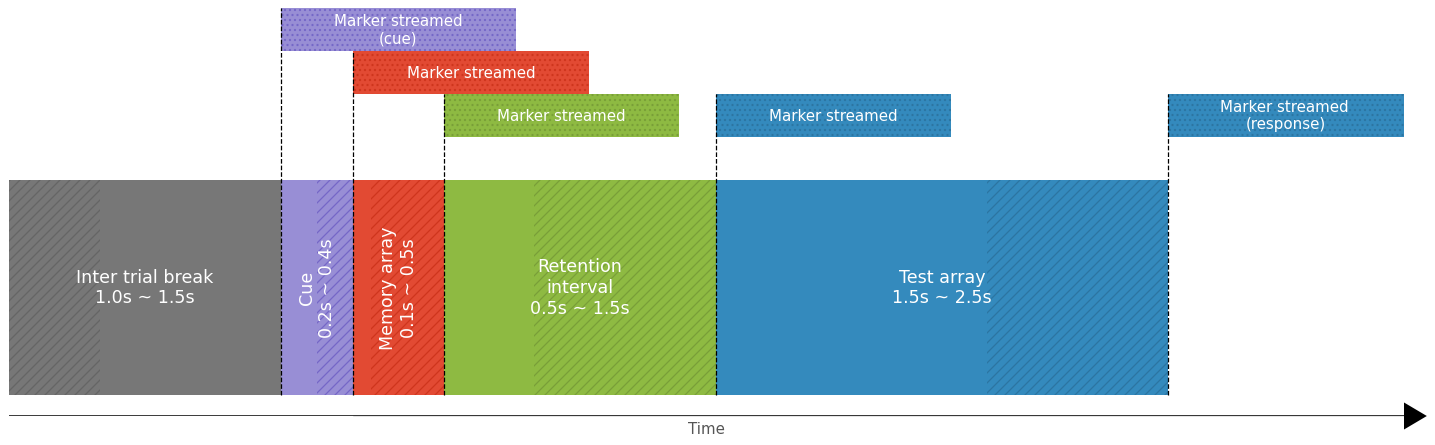
\includegraphics[width=1\textwidth]{Appendix/databases/Figures/vwm-paradigm.png}
\par\end{centering}
\caption{\gls*{VWM} paradigm implementation with markers indicators.}
\label{}
\end{figure}


%======================================================================
\section{Stimuli presentation}
All stimuli are presented on a computer screen situated 120 cm away from the subject. The stimulus arrays appear within two $7.2^{\circ}$ × $13.15^{\circ}$ rectangular regions that are centered $5.4^{\circ}$ to the left and right of a central fixation cross on a gray background (the symbol $\circ$ stands for degrees of visual angle \cite{newsome1972visual, haeuslschmid2017recognition}. Each colored square ($1.17^{\circ}$ × $1.17^{\circ}$) is randomly selected from a set of seven colors (red, blue, violet, green, yellow, black and white). A given color can appear no more than twice within an array. Stimulus positions were randomized  on each trial, with the constraint that the distance between squares within a hemifield was at least $3.5^{\circ}$ (center to center) \cite{villena2020data}.

\begin{figure}[H]
\begin{centering}
% \includesvg[width=0.8\textwidth]{Cap4/Figures/transformer.svg}
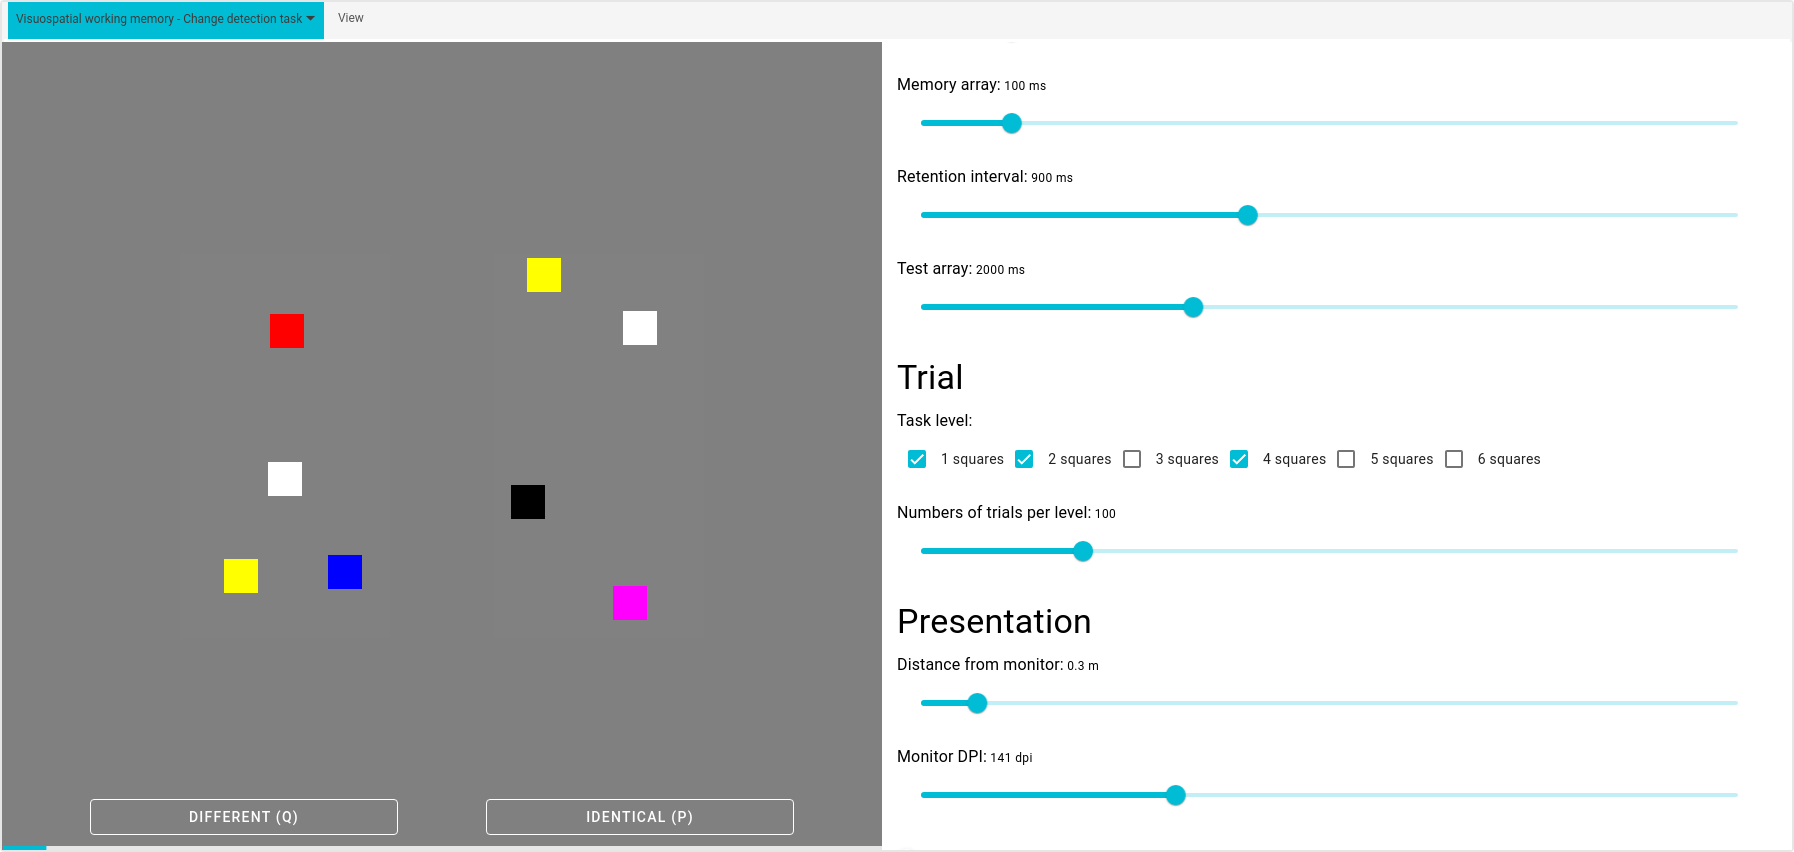
\includegraphics[width=1\textwidth]{Appendix/databases/Figures/vwm-delivery.png}
\par\end{centering}
\caption{\gls*{VWM} stimuli delivery interface.}
\label{}
\end{figure}


%======================================================================
\section{Neurofeedback} \label{appendix:neurofeedback}

Neurofeedback is attracting renewed interest as a method to self-regulate one’s own brain activity to directly alter the underlying neural mechanisms of cognition and behavior. It not only promises new avenues as a method for cognitive enhancement in healthy subjects, but also as a therapeutic tool. In the current article, we present a review tutorial discussing key aspects relevant to the development of EEG neurofeedback studies. In addition, the putative mechanisms underlying neurofeedback learning are considered. We highlight both aspects relevant for the practical application of neurofeedback as well as rather theoretical considerations related to the development of new generation protocols. Important characteristics regarding the set-up of a neurofeedback protocol are outlined in a step-by-step way. All these practical and theoretical considerations are illustrated based on a protocol and results of a frontal-midline theta up-regulation training for the improvement of executive functions. Not least, assessment criteria for the validation of neurofeedback studies as well as general guidelines for the evaluation of training efficacy are discussed \cite{enriquez2017eeg}.

\begin{figure}[H]
\begin{centering}
% \includesvg[width=0.8\textwidth]{Cap4/Figures/transformer.svg}
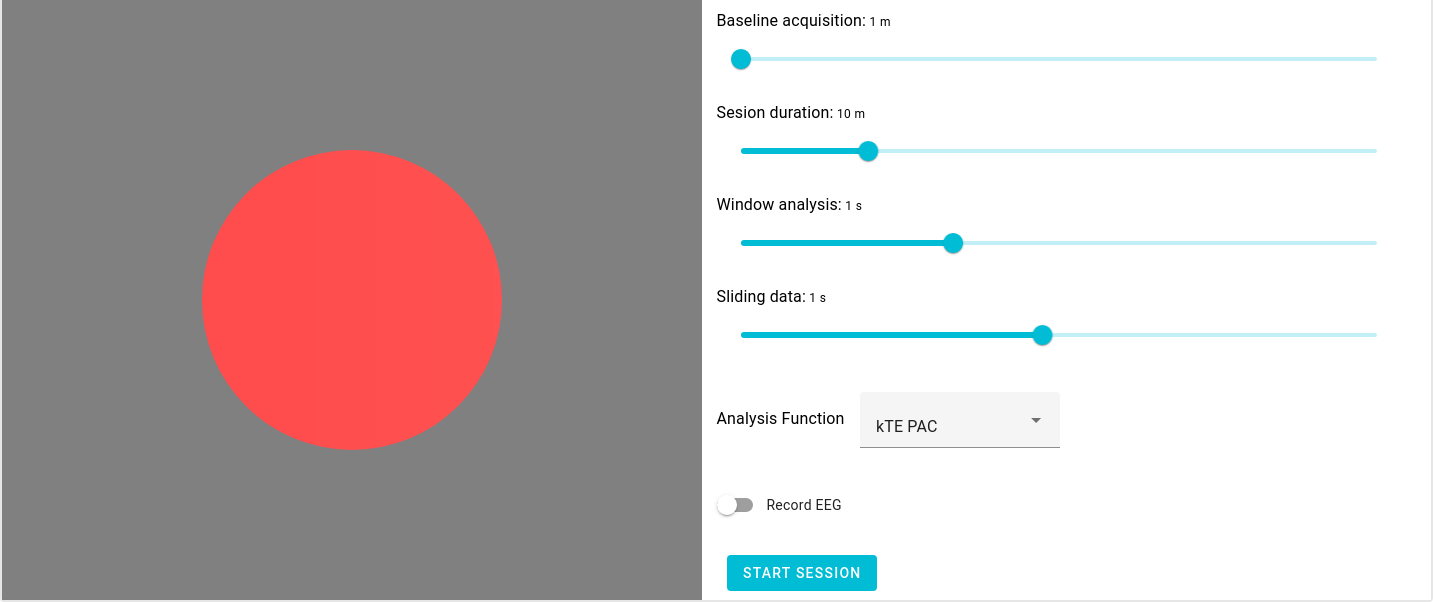
\includegraphics[width=1\textwidth]{Appendix/databases/Figures/vwm-neurofeedback.png}
\par\end{centering}
\caption{\gls*{VWM} neurofeedback dash board.}
\label{}
\end{figure}